
\documentclass[a4paper,11pt]{article}
\usepackage{geometry}
\geometry{margin=2cm}
\usepackage{booktabs}
\usepackage{graphicx}
\usepackage{amsmath}
\usepackage{siunitx}
\usepackage{caption}
\usepackage{times}
\usepackage[utf8]{inputenc}
\usepackage{tocloft}
\usepackage{pdflscape} % Untuk mendukung landscape

\title{Spectral Simulation Report}
\author{Automated Analysis}
\date{\today}

\begin{document}

\maketitle
\tableofcontents
\clearpage

\section{Introduction}
This report presents the results of spectral simulations derived from HDF5 dataset analysis. Each sample includes a spectral plot displayed in a full horizontal page and a detailed table summarizing the initial composition, actual positions, total pixels, and signal-to-noise ratio (SNR), along with simulation parameters such as temperature and electron density.


\section{Sample: 8427}
\subsection{Simulation Parameters}
\begin{table}[h!]
    \centering
    \begin{tabular}{ll}
        \toprule
        \textbf{Parameter} & \textbf{Value} \\
        \midrule
        Temperature ($T$) & 14798 \,\si{K} \\
        Electron Density ($n_e$) & 3.94e+17 \,\si{cm^-3} \\
        Total Pixels & 4096 \\
        Signal-to-Noise Ratio (SNR) & 35.85 \\
        \bottomrule
    \end{tabular}
    \caption{Simulation parameters and additional metrics for sample 8427.}
    \label{tab:params_8427}
\end{table}

\subsection{Composition Analysis}
\begin{table}[h!]
    \centering
    \begin{tabular}{lcc}
        \toprule
        \textbf{Element} & \textbf{Initial Composition (\%)} & \textbf{Actual Positions} \\
        \midrule
        Al & 0.00 & 0.0 \\
        Ar & 0.00 & 0.0 \\
        C & 2.58 & 848.0 \\
        Ca & 9.44 & 150.0 \\
        Cl & 3.60 & 35.0 \\
        Co & 8.85 & 1404.0 \\
        Cr & 6.09 & 397.0 \\
        Fe & 10.57 & 2790.0 \\
        Mg & 7.42 & 358.0 \\
        Mn & 12.87 & 706.0 \\
        N & 13.65 & 861.0 \\
        Na & 1.92 & 325.0 \\
        Ni & 1.72 & 478.0 \\
        O & 0.00 & 0.0 \\
        S & 9.73 & 228.0 \\
        Si & 11.57 & 223.0 \\
        Ti & 0.00 & 0.0 \\
        background & N/A & 471.0 \\

        \midrule
        \textbf{Total Positions} & & 9274.0 \\
        \bottomrule
    \end{tabular}
    \caption{Composition analysis for sample 8427.}
    \label{tab:comp_8427}
\end{table}

\subsection{Spectral Plot}
\begin{figure}[p]
    \begin{landscape}
        \centering
        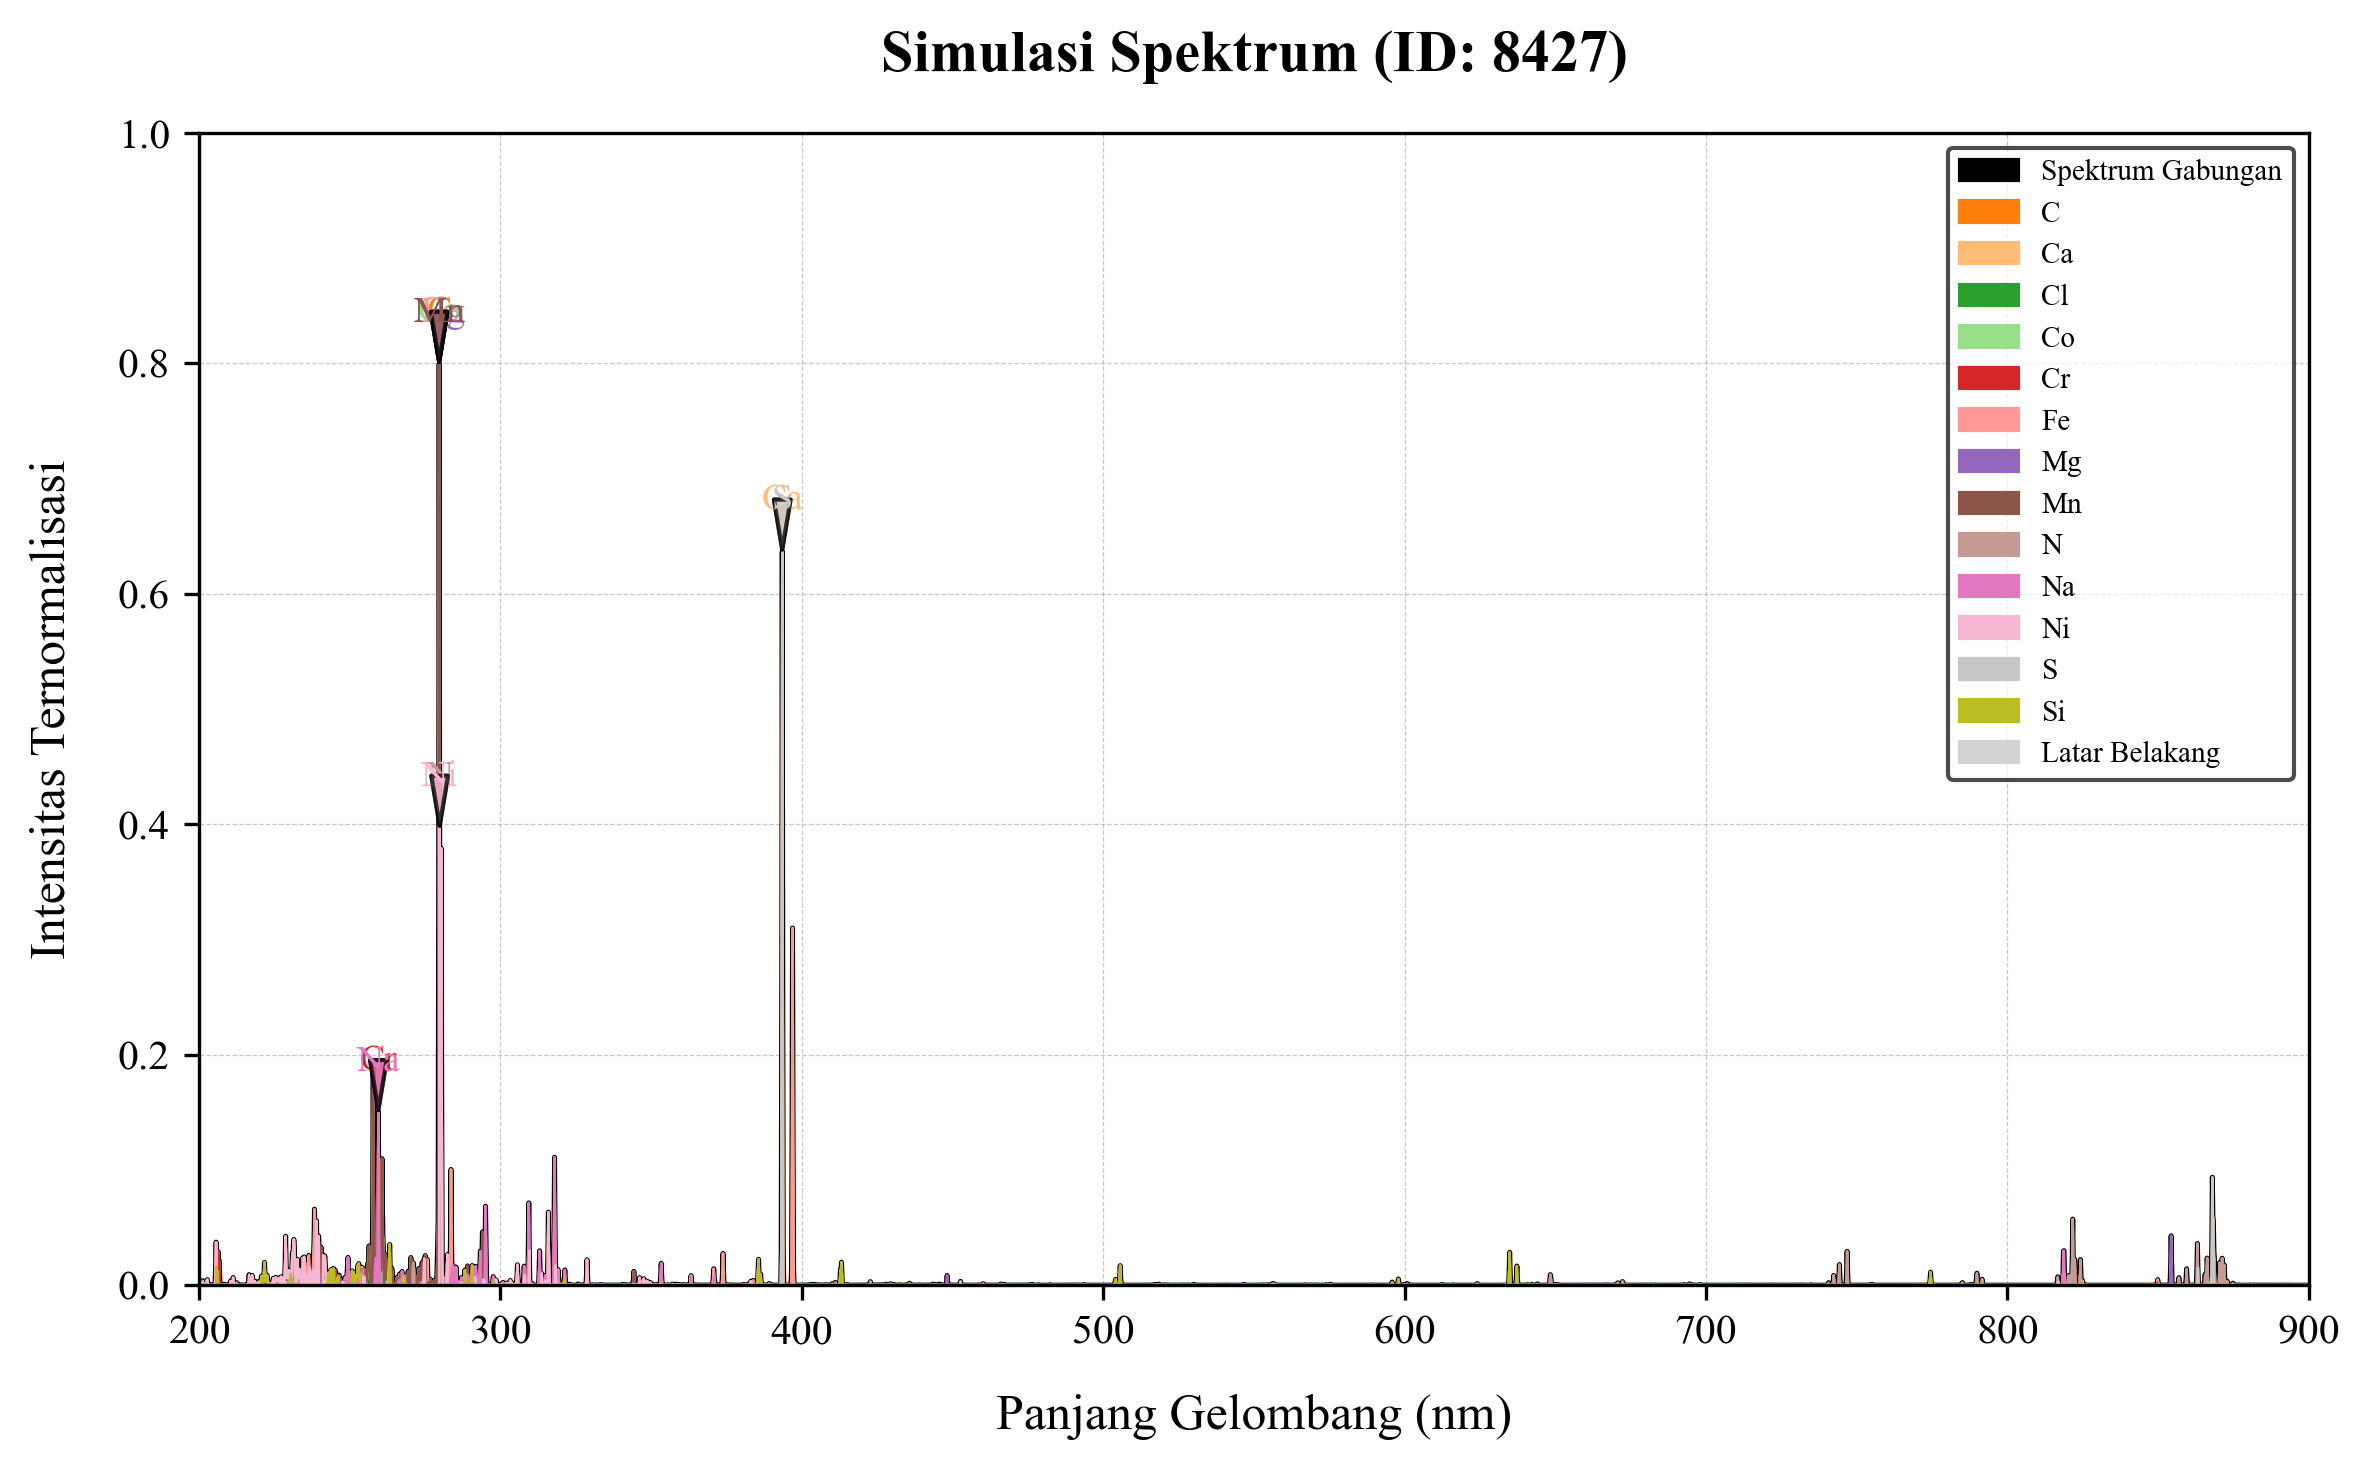
\includegraphics[width=1.2\textwidth, angle=90]{spectrum_8427.png}
        \caption{Spectral simulation plot for sample 8427 in full horizontal layout.}
        \label{fig:spectrum_8427}
    \end{landscape}
\end{figure}

\clearpage

\section{Sample: 5347}
\subsection{Simulation Parameters}
\begin{table}[h!]
    \centering
    \begin{tabular}{ll}
        \toprule
        \textbf{Parameter} & \textbf{Value} \\
        \midrule
        Temperature ($T$) & 11869 \,\si{K} \\
        Electron Density ($n_e$) & 5.99e+15 \,\si{cm^-3} \\
        Total Pixels & 4096 \\
        Signal-to-Noise Ratio (SNR) & 30.12 \\
        \bottomrule
    \end{tabular}
    \caption{Simulation parameters and additional metrics for sample 5347.}
    \label{tab:params_5347}
\end{table}

\subsection{Composition Analysis}
\begin{table}[h!]
    \centering
    \begin{tabular}{lcc}
        \toprule
        \textbf{Element} & \textbf{Initial Composition (\%)} & \textbf{Actual Positions} \\
        \midrule
        Al & 10.52 & 462.0 \\
        Ar & 8.28 & 727.0 \\
        C & 3.88 & 447.0 \\
        Ca & 0.35 & 150.0 \\
        Cl & 10.96 & 35.0 \\
        Co & 7.63 & 1404.0 \\
        Cr & 11.04 & 397.0 \\
        Fe & 10.10 & 2765.0 \\
        Mg & 2.96 & 352.0 \\
        Mn & 1.94 & 706.0 \\
        N & 8.19 & 547.0 \\
        Na & 1.34 & 322.0 \\
        Ni & 2.04 & 476.0 \\
        O & 4.83 & 217.0 \\
        S & 7.25 & 228.0 \\
        Si & 4.53 & 223.0 \\
        Ti & 4.16 & 1186.0 \\
        background & N/A & 371.0 \\

        \midrule
        \textbf{Total Positions} & & 11015.0 \\
        \bottomrule
    \end{tabular}
    \caption{Composition analysis for sample 5347.}
    \label{tab:comp_5347}
\end{table}

\subsection{Spectral Plot}
\begin{figure}[p]
    \begin{landscape}
        \centering
        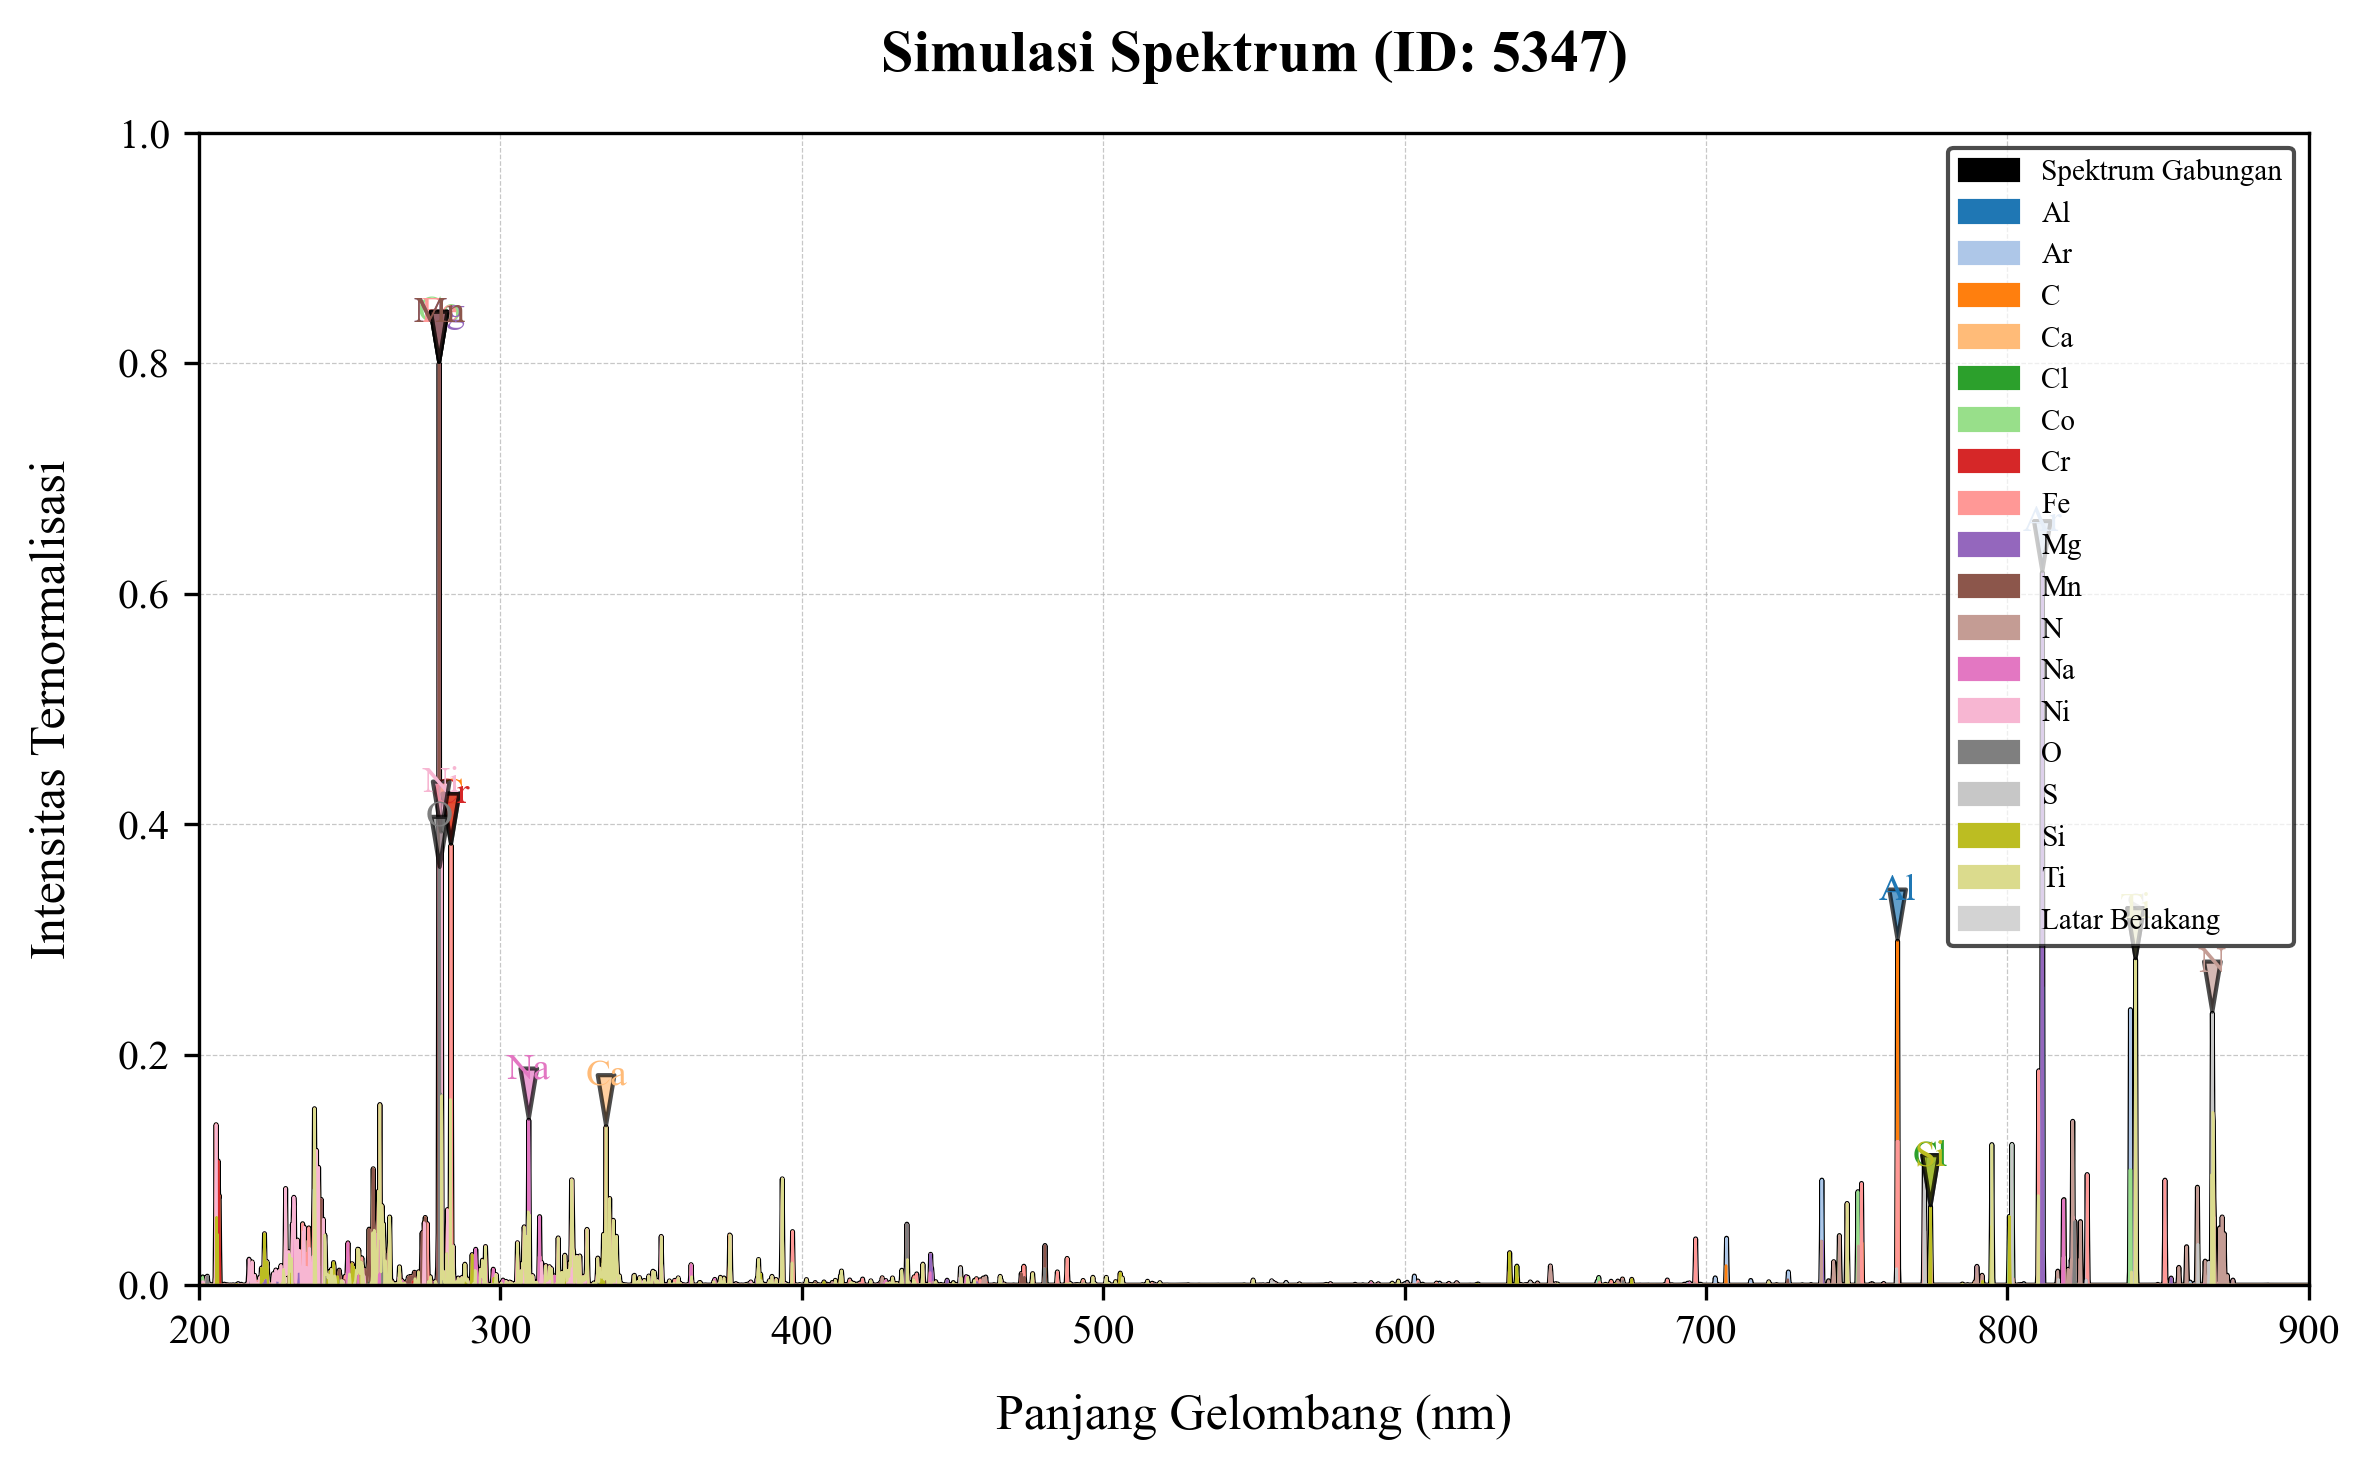
\includegraphics[width=1.2\textwidth, angle=90]{spectrum_5347.png}
        \caption{Spectral simulation plot for sample 5347 in full horizontal layout.}
        \label{fig:spectrum_5347}
    \end{landscape}
\end{figure}

\clearpage

\section{Sample: 8671}
\subsection{Simulation Parameters}
\begin{table}[h!]
    \centering
    \begin{tabular}{ll}
        \toprule
        \textbf{Parameter} & \textbf{Value} \\
        \midrule
        Temperature ($T$) & 8232 \,\si{K} \\
        Electron Density ($n_e$) & 2.01e+16 \,\si{cm^-3} \\
        Total Pixels & 4096 \\
        Signal-to-Noise Ratio (SNR) & 36.83 \\
        \bottomrule
    \end{tabular}
    \caption{Simulation parameters and additional metrics for sample 8671.}
    \label{tab:params_8671}
\end{table}

\subsection{Composition Analysis}
\begin{table}[h!]
    \centering
    \begin{tabular}{lcc}
        \toprule
        \textbf{Element} & \textbf{Initial Composition (\%)} & \textbf{Actual Positions} \\
        \midrule
        Al & 4.51 & 341.0 \\
        Ar & 9.94 & 725.0 \\
        C & 5.46 & 224.0 \\
        Ca & 10.78 & 150.0 \\
        Cl & 3.35 & 12.0 \\
        Co & 10.37 & 1404.0 \\
        Cr & 8.39 & 397.0 \\
        Fe & 4.28 & 2725.0 \\
        Mg & 0.00 & 0.0 \\
        Mn & 8.14 & 706.0 \\
        N & 2.70 & 396.0 \\
        Na & 4.87 & 326.0 \\
        Ni & 5.27 & 478.0 \\
        O & 9.50 & 130.0 \\
        S & 1.94 & 39.0 \\
        Si & 7.96 & 220.0 \\
        Ti & 2.55 & 1183.0 \\
        background & N/A & 463.0 \\

        \midrule
        \textbf{Total Positions} & & 9919.0 \\
        \bottomrule
    \end{tabular}
    \caption{Composition analysis for sample 8671.}
    \label{tab:comp_8671}
\end{table}

\subsection{Spectral Plot}
\begin{figure}[p]
    \begin{landscape}
        \centering
        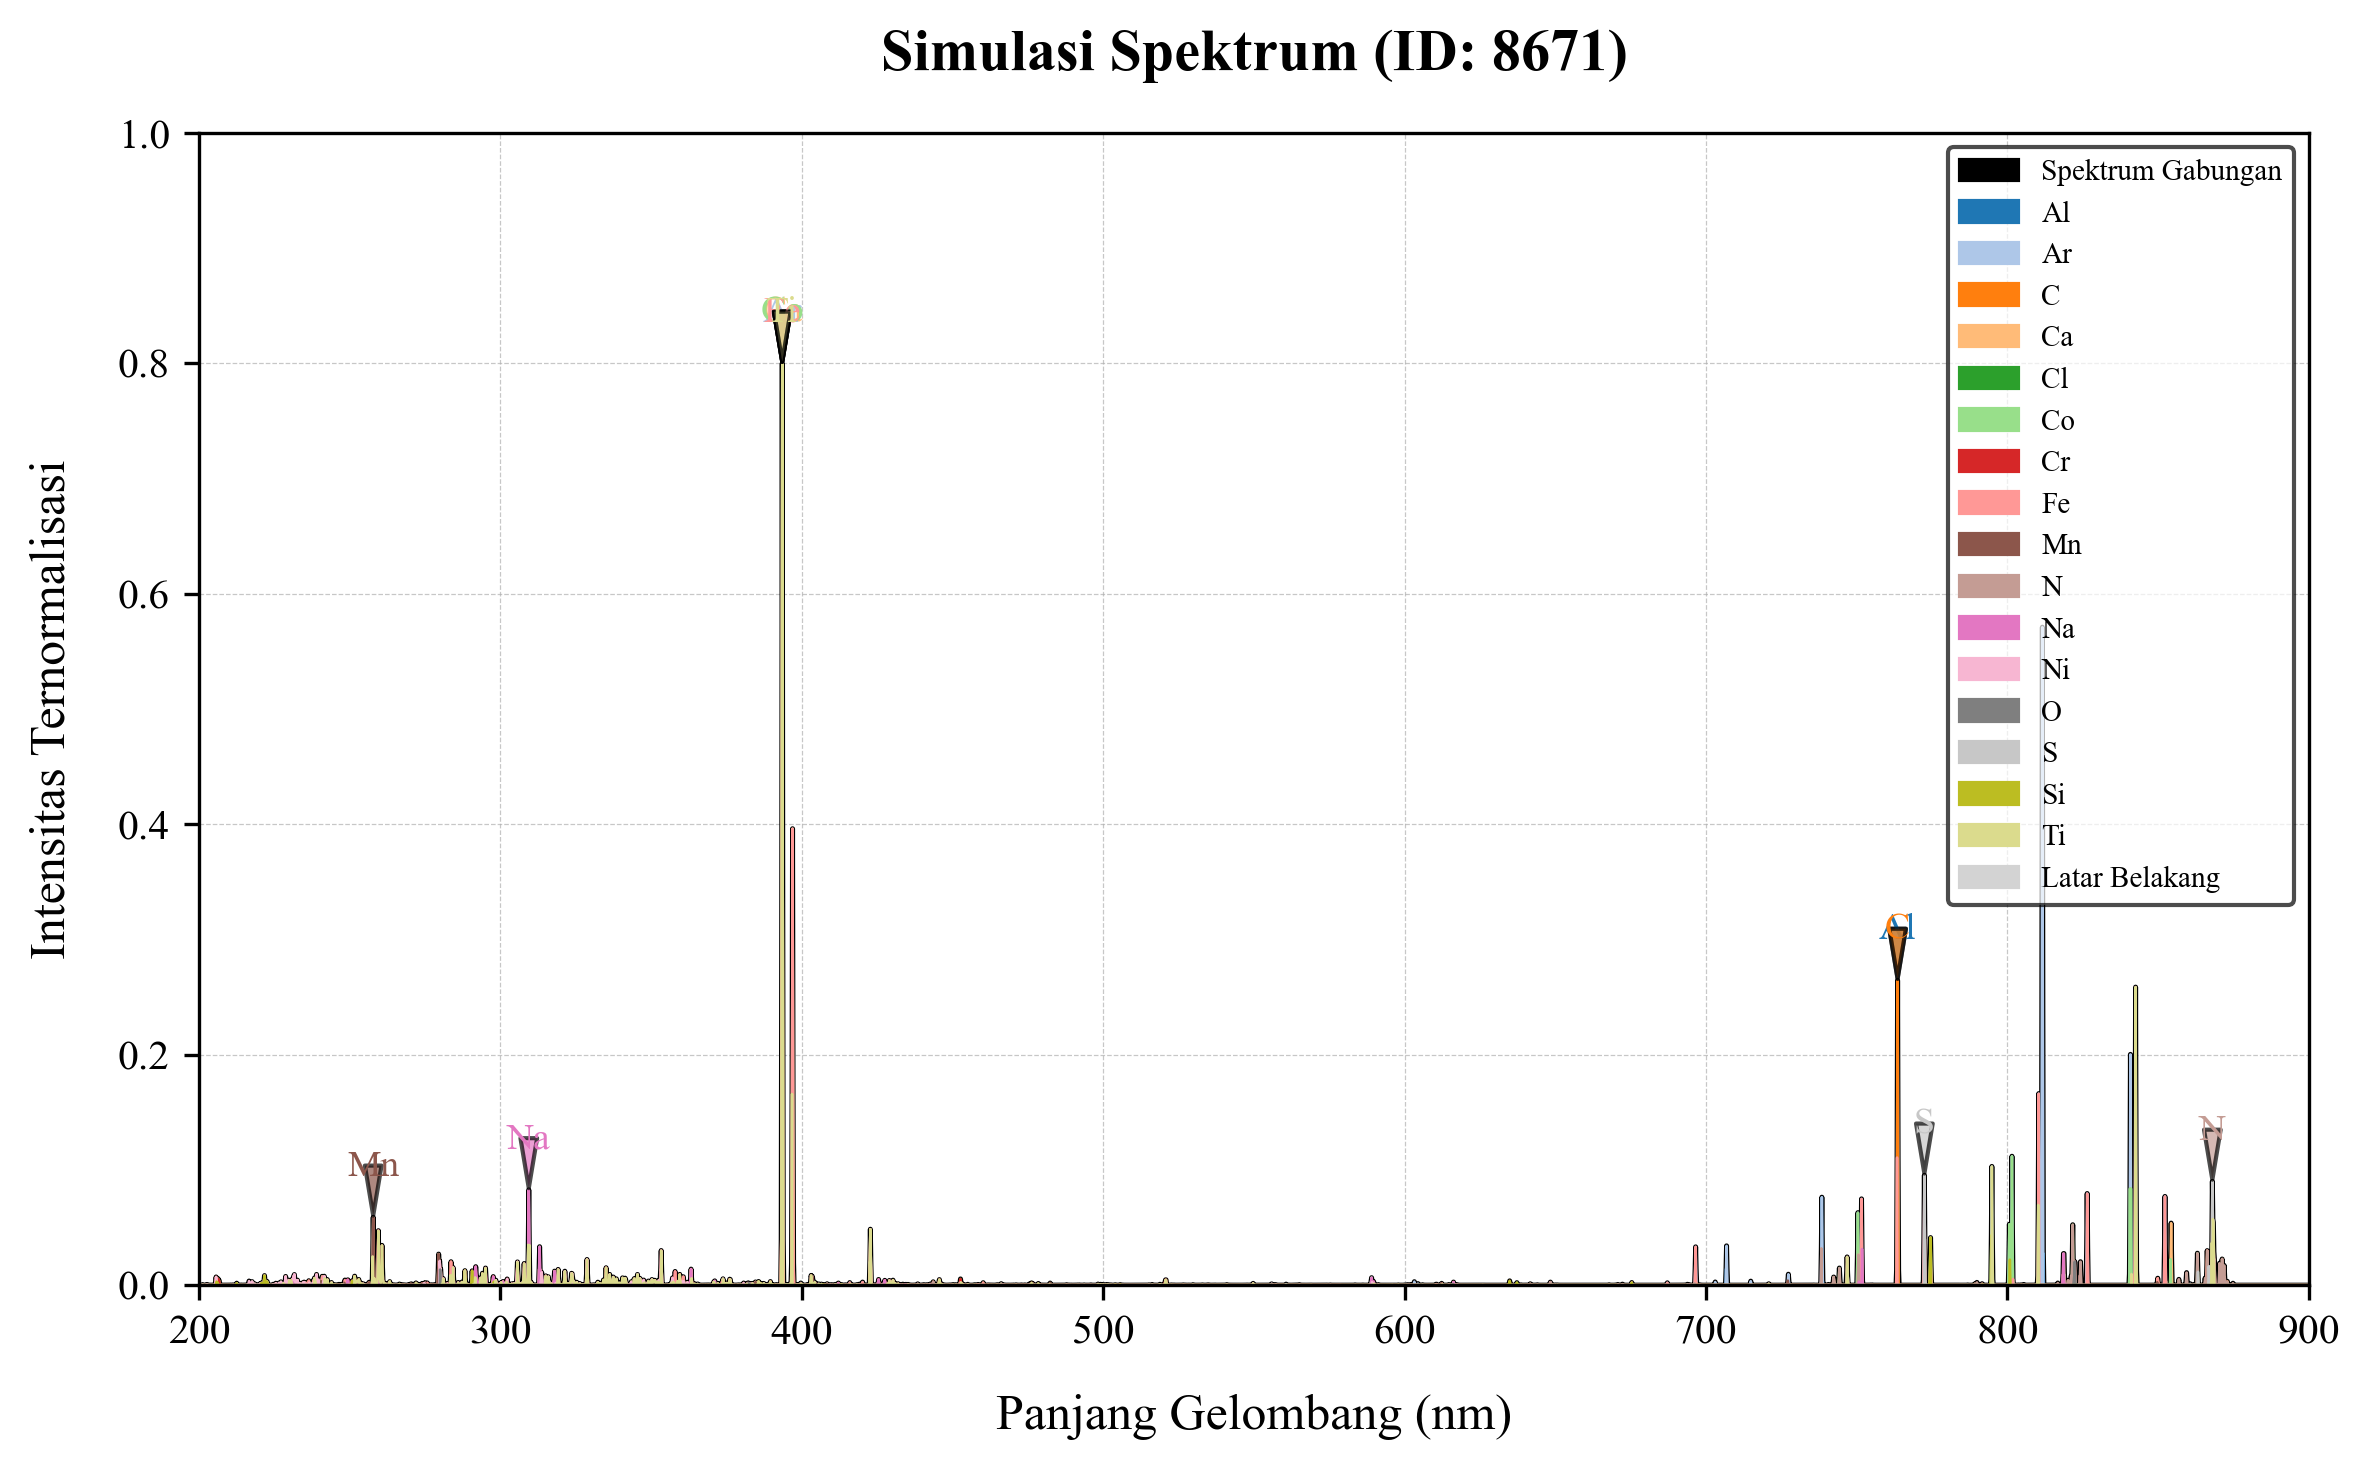
\includegraphics[width=1.2\textwidth, angle=90]{spectrum_8671.png}
        \caption{Spectral simulation plot for sample 8671 in full horizontal layout.}
        \label{fig:spectrum_8671}
    \end{landscape}
\end{figure}

\clearpage

\section{Sample: 7682}
\subsection{Simulation Parameters}
\begin{table}[h!]
    \centering
    \begin{tabular}{ll}
        \toprule
        \textbf{Parameter} & \textbf{Value} \\
        \midrule
        Temperature ($T$) & 6414 \,\si{K} \\
        Electron Density ($n_e$) & 2.26e+17 \,\si{cm^-3} \\
        Total Pixels & 4096 \\
        Signal-to-Noise Ratio (SNR) & 35.34 \\
        \bottomrule
    \end{tabular}
    \caption{Simulation parameters and additional metrics for sample 7682.}
    \label{tab:params_7682}
\end{table}

\subsection{Composition Analysis}
\begin{table}[h!]
    \centering
    \begin{tabular}{lcc}
        \toprule
        \textbf{Element} & \textbf{Initial Composition (\%)} & \textbf{Actual Positions} \\
        \midrule
        Al & 9.96 & 149.0 \\
        Ar & 7.60 & 255.0 \\
        C & 4.24 & 188.0 \\
        Ca & 7.17 & 150.0 \\
        Cl & 1.74 & 12.0 \\
        Co & 3.86 & 828.0 \\
        Cr & 6.15 & 397.0 \\
        Fe & 3.71 & 2122.0 \\
        Mg & 0.85 & 146.0 \\
        Mn & 7.49 & 621.0 \\
        N & 6.36 & 396.0 \\
        Na & 4.80 & 330.0 \\
        Ni & 10.64 & 478.0 \\
        O & 2.01 & 12.0 \\
        S & 4.43 & 25.0 \\
        Si & 6.91 & 156.0 \\
        Ti & 12.07 & 1181.0 \\
        background & N/A & 926.0 \\

        \midrule
        \textbf{Total Positions} & & 8372.0 \\
        \bottomrule
    \end{tabular}
    \caption{Composition analysis for sample 7682.}
    \label{tab:comp_7682}
\end{table}

\subsection{Spectral Plot}
\begin{figure}[p]
    \begin{landscape}
        \centering
        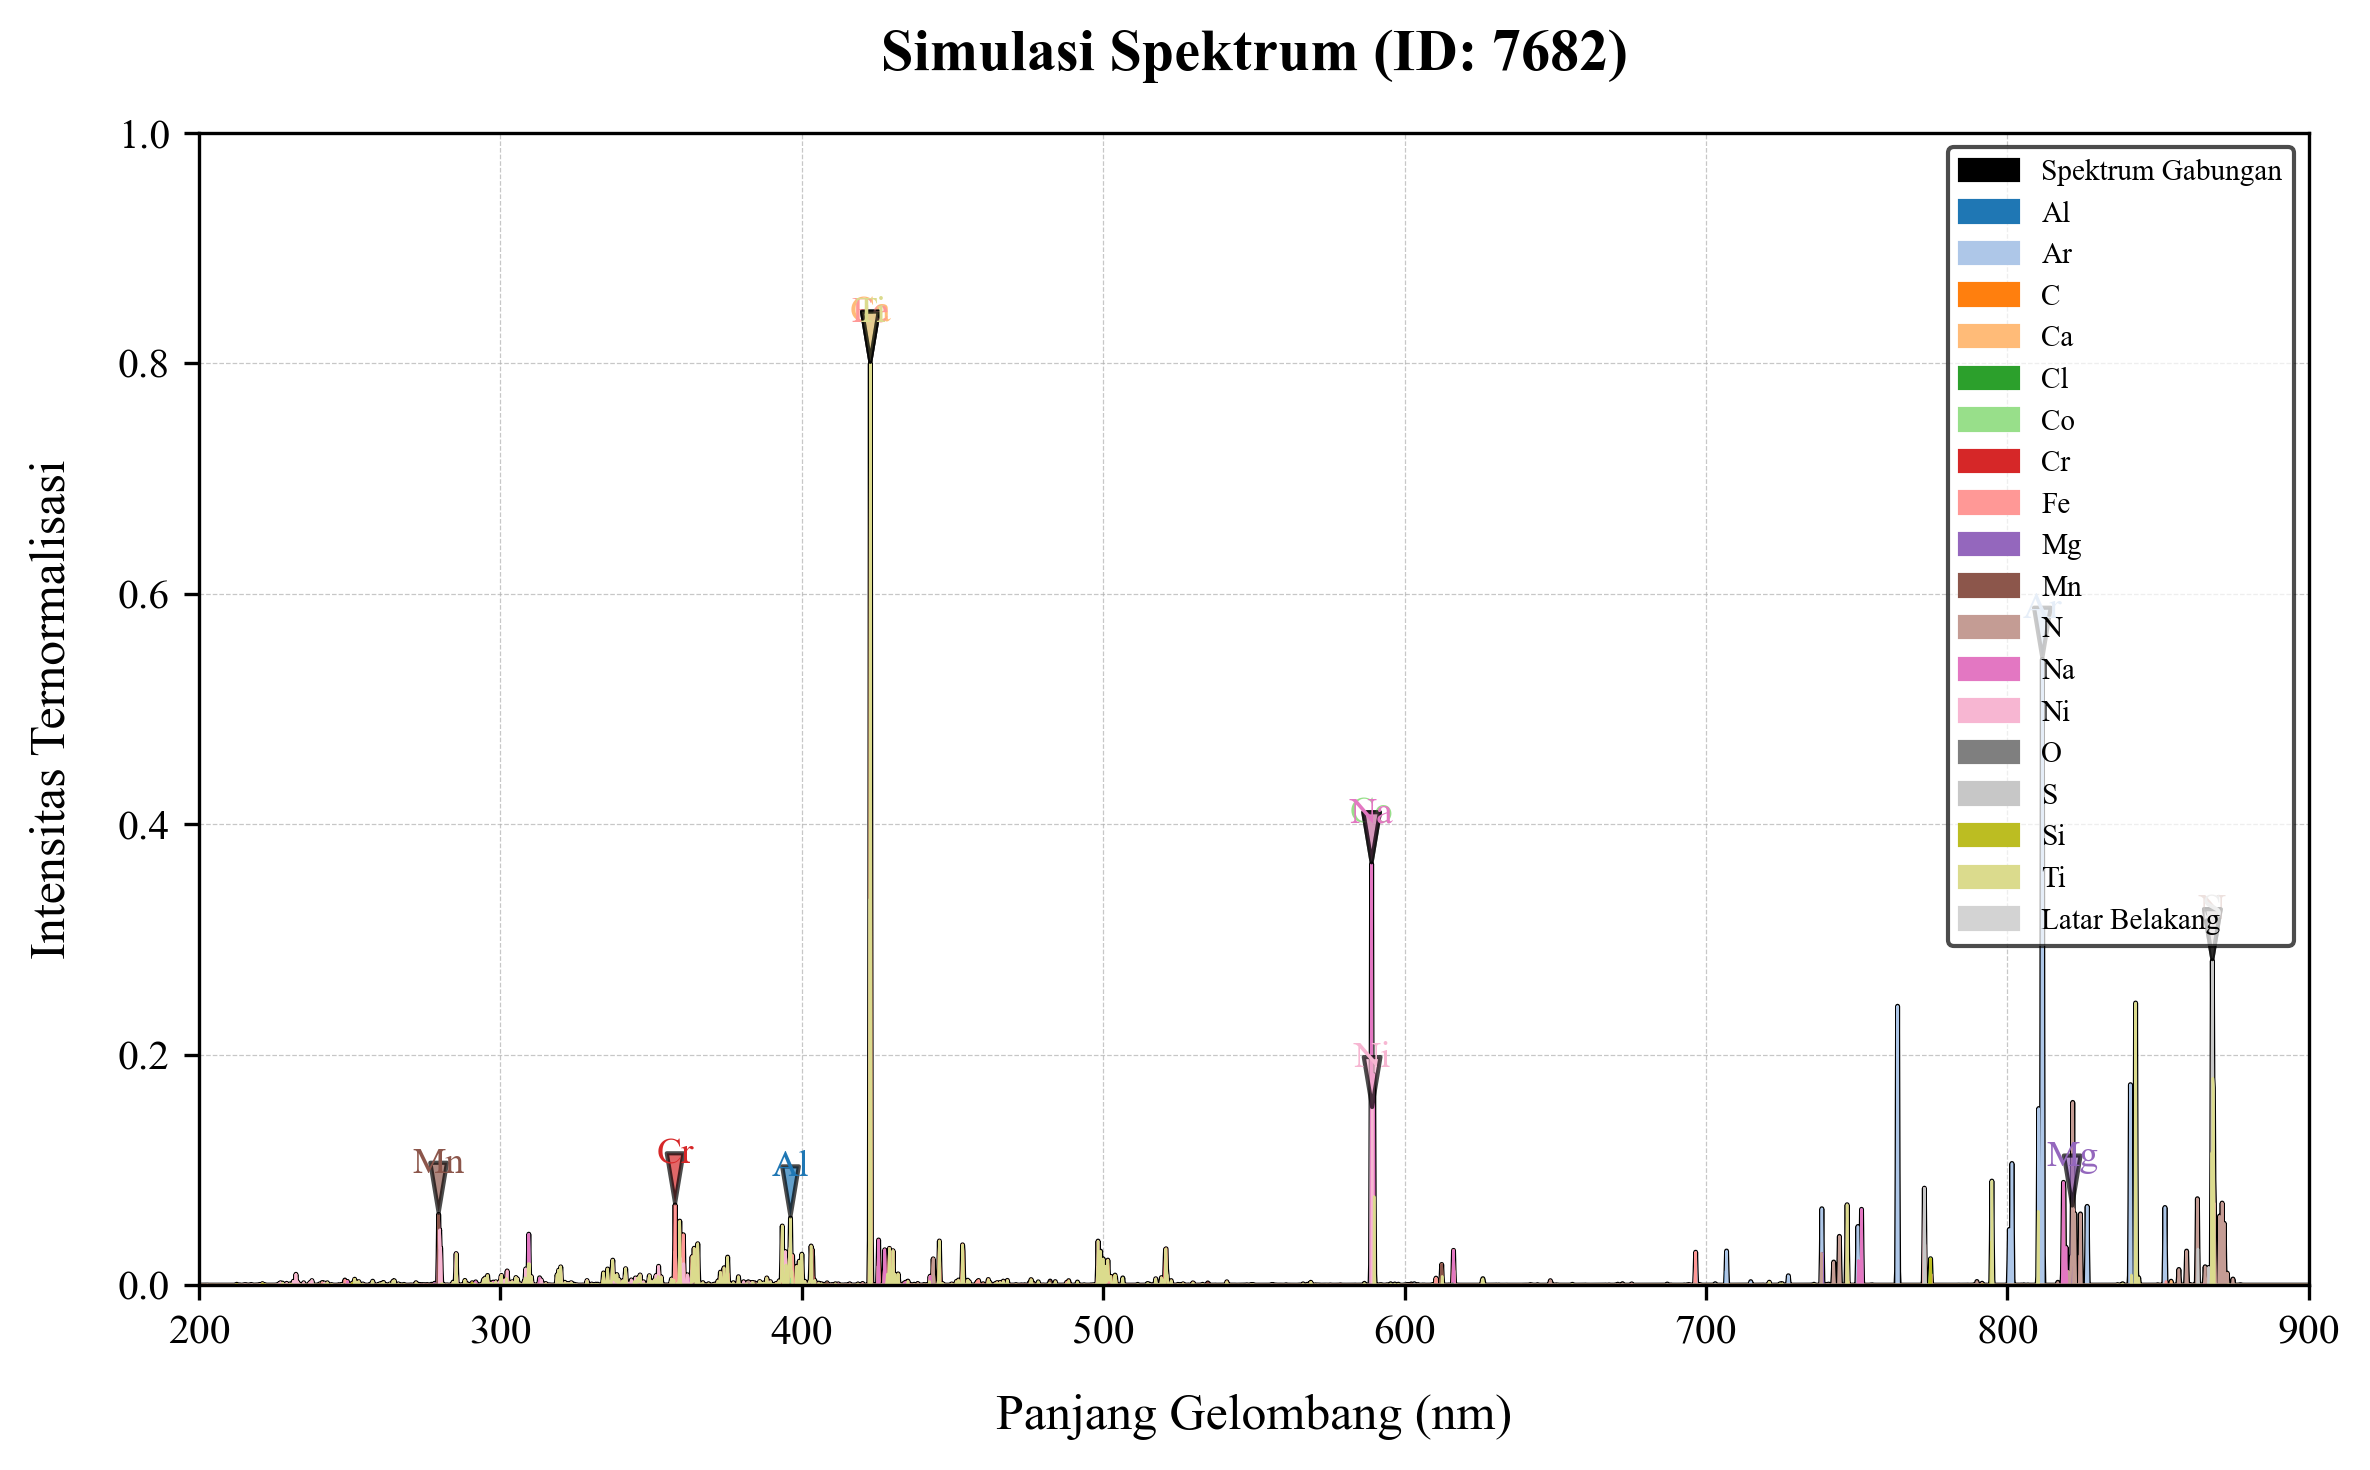
\includegraphics[width=1.2\textwidth, angle=90]{spectrum_7682.png}
        \caption{Spectral simulation plot for sample 7682 in full horizontal layout.}
        \label{fig:spectrum_7682}
    \end{landscape}
\end{figure}

\clearpage

\section{Sample: 18066}
\subsection{Simulation Parameters}
\begin{table}[h!]
    \centering
    \begin{tabular}{ll}
        \toprule
        \textbf{Parameter} & \textbf{Value} \\
        \midrule
        Temperature ($T$) & 5101 \,\si{K} \\
        Electron Density ($n_e$) & 1.00e+18 \,\si{cm^-3} \\
        Total Pixels & 4096 \\
        Signal-to-Noise Ratio (SNR) & 43.58 \\
        \bottomrule
    \end{tabular}
    \caption{Simulation parameters and additional metrics for sample 18066.}
    \label{tab:params_18066}
\end{table}

\subsection{Composition Analysis}
\begin{table}[h!]
    \centering
    \begin{tabular}{lcc}
        \toprule
        \textbf{Element} & \textbf{Initial Composition (\%)} & \textbf{Actual Positions} \\
        \midrule
        Al & 0.00 & 0.0 \\
        Ar & 0.00 & 0.0 \\
        C & 0.00 & 0.0 \\
        Ca & 20.30 & 145.0 \\
        Cl & 12.50 & 12.0 \\
        Co & 1.44 & 623.0 \\
        Cr & 21.64 & 397.0 \\
        Fe & 0.00 & 0.0 \\
        Mg & 2.48 & 125.0 \\
        Mn & 11.99 & 359.0 \\
        N & 0.00 & 0.0 \\
        Na & 9.65 & 323.0 \\
        Ni & 17.99 & 466.0 \\
        O & 0.00 & 0.0 \\
        S & 1.42 & 25.0 \\
        Si & 0.58 & 83.0 \\
        Ti & 0.00 & 0.0 \\
        background & N/A & 2341.0 \\

        \midrule
        \textbf{Total Positions} & & 4899.0 \\
        \bottomrule
    \end{tabular}
    \caption{Composition analysis for sample 18066.}
    \label{tab:comp_18066}
\end{table}

\subsection{Spectral Plot}
\begin{figure}[p]
    \begin{landscape}
        \centering
        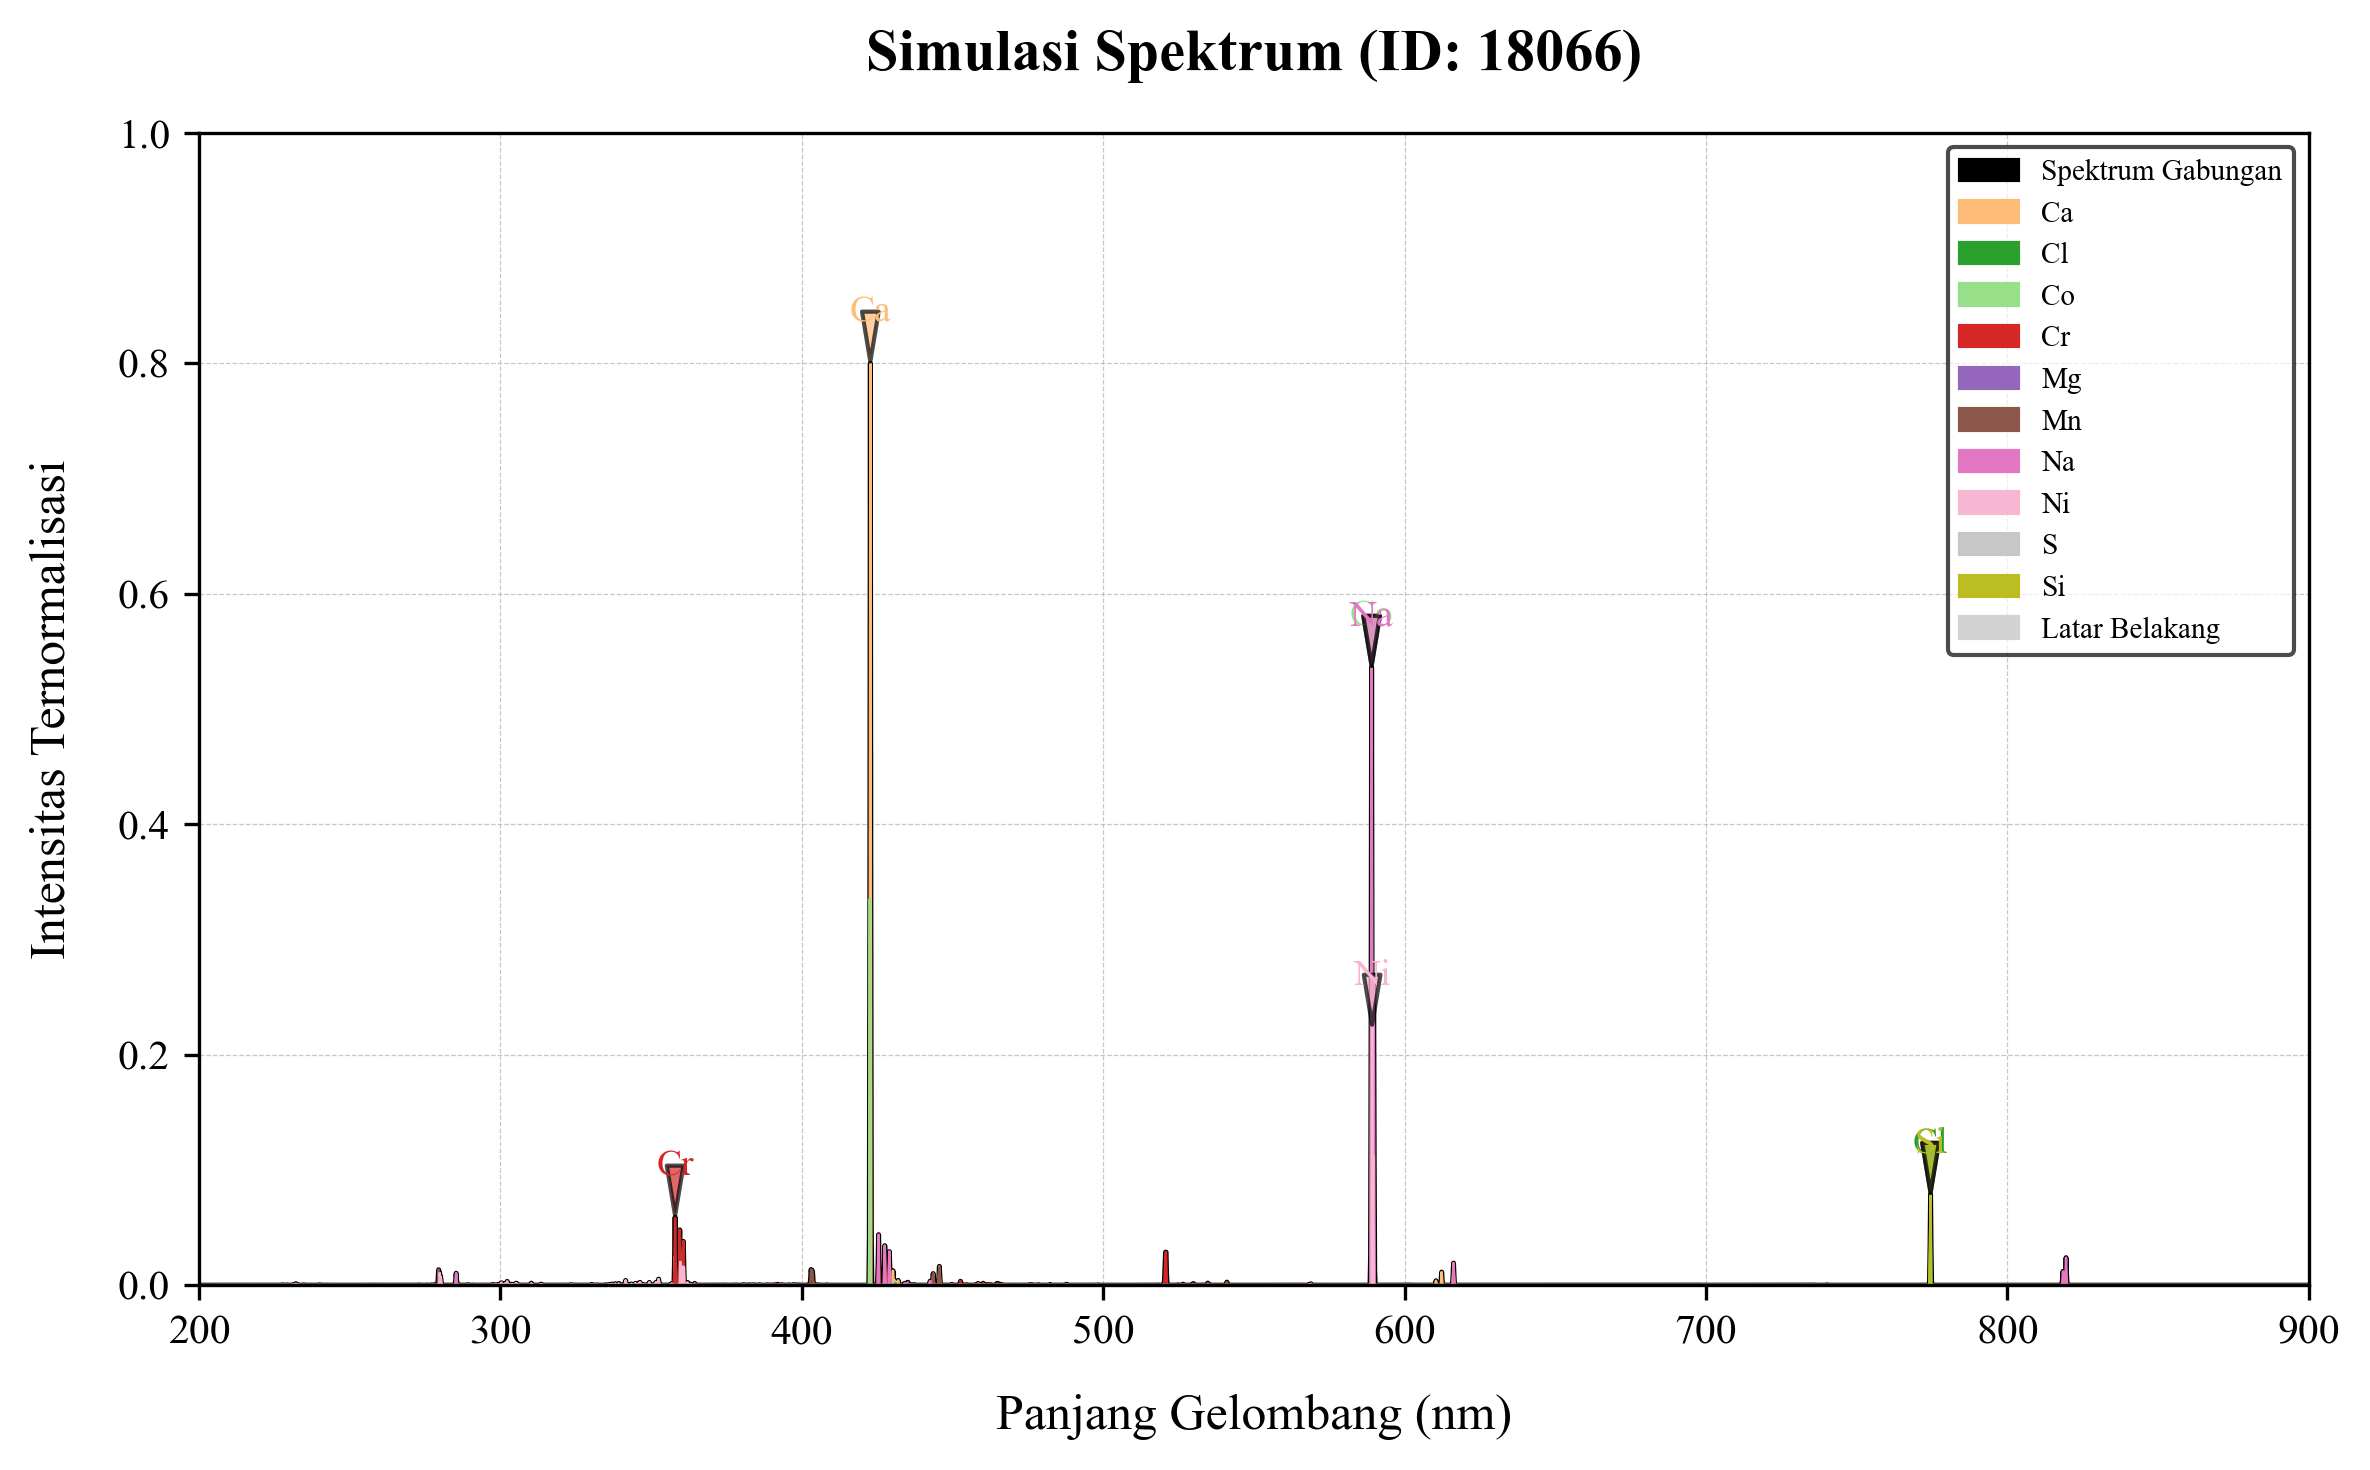
\includegraphics[width=1.2\textwidth, angle=90]{spectrum_18066.png}
        \caption{Spectral simulation plot for sample 18066 in full horizontal layout.}
        \label{fig:spectrum_18066}
    \end{landscape}
\end{figure}

\clearpage

\end{document}
